Der Hauptdetektor dieser Analyse ist das EMCal.
In einem Abstand von 4,5m vom prim\"aren Vertex deckt das EMCal einen Azimuthalwinkelbereich von $\phi=107^{\circ}$ und einen Rapidit\"atsbreich von $ |\eta| \leq 0,7$ ab.
Aufgrund von Detektormaterial und Tr\"agerstrukturen zwischen dem prim\"aren Vertex und dem EMCal k\"onnen Teilchen abgelenkt werden oder Photonen in ein Elektron-Positron-Paar konvertieren.
Die Konvertierung von Photonen ist besonders zu beachten, da in dieser Analyse $\pi^{0}$, welche in zwei Photonen zerfallen, rekonstruiert werden.
\newline
Das EMCal besteht aus zw\"olf sogenannten Supermodulen, zehn normal gro{\ss}e und zwei Eindrittel gro{\ss}e.
Ein normal gro{\ss}es Supermodul unterteilt sich in 24 sogenannte Streifenmodule, welche wiederum aus 12 Modulen zusammengesetzt sind.
Jedes Modul beinhaltet 4 Zellen, womit das EMCal aus insgesamt 12288 Zellen besteht.
Die Zellen sind f\"ur das Detektieren und Messen der Energie von haupts\"achlich Photonen, Elektronen und Positronen verantwortlich.
Daf\"ur besteht eine einzelne Zelle aus abwechselnd 77 Szintillatoren- und 76 Bleischichten.
In den Bleischichten entstehen sogenannten elektromagnetische Schauer, indem eintreffende Photonen durch Paarerzeugung in ein Elektron und ein Positron zerfallen, welche wiederum durch Bremsstrahlung weitere Photonen abstrahlen.
Die Szintillatoren wandeln die hochenergetischen Photonen in ein messbares Lichtsignal.
Alle Szintillatorschichten einer Zelle sind \"uber ein Glasfaserkabel mit einem Photomultiplier verbunden.
Der Photomultiplier wandelt das Lichtsignal in ein elektrisches Signal, welches proportional zu gespeicherten Energie der Zelle ist.
\newline
Jeder elektromagnetischer Schauer besitzt eine gewisse Ausdehnung, welche \"uber den sogenannten Moli\`ere-Radius $R_{\text{M}}$ definiert ist.
Der Moli\`ere-Radius gibt den Radius passend zu einem Zylinder an, in welchem 90\% der gesamten Energie eines Schauers vom Detektor absorbiert wurde.
F\"ur das EMCal betr\"agt der Moli\`ere-Radius $R_{\text{M}} = 3,7 cm$, womit sich eine Kreisfl\"ache von ca. $43 cm^{2}$ ergibt.
Die einzelnen Zellen des EMCal hingegen haben eine quadratische Fl\"ache von $36 cm^{2}$. 
Der Schauer eines einzelnen Teilchens erstreckt sich also \"uber mehrere Zellen, weshalb mehrere Zellen durch eine Algorithmus zu sogenannten \textit{Clustern} zusammengefasst werden.
Algorithmen zur Rekonstruktion von \textit{Clustern} hei{\ss}en \textit{Clusterizer}.
In der hier vorliegenden Analyse wird der sogenannte v2-\textit{Clusterizer} verwendet.
Dieser sucht zun\"achst nach der Zelle mit der gr\"o{\ss}ten deponierten Energie, welche noch keinem \textit{Cluster} angeh\"ohrt und eine gewisse Schwellenenergie besitzt.
Von dieser Startzelle ausgehend werden die Nachbarzellen abgesucht und zum \textit{Cluster} hinzugef\"ugt, wenn sie eine gewisse Mindestenergie \"uberschreiten und ebefalls keinem weiteren \textit{Cluster} zugeordnet sind.
Dies Suche nach Nachbarzellen geschieht dabei iterativ solange, bis keine Nachbarzellen die n\"otigen Kriterien erf\"ullen um dem \textit{Cluster} hinzugef\"ugt zu werden.
Anschlie{\ss}end wird eine neue Startzelle f\"ur ein neues \textit{Cluster} gesucht und der Prozess beginnt von vorne.

\begin{figure}[thp]
\centering
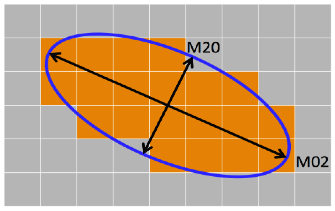
\includegraphics[width=.35\linewidth]{m02&m20.png}
\caption{Schematische Darstellung eines \textit{Clusters}. Die Ellipsenhalbachsen M20 und M02 definieren eine Ellipse, welche alle orange markierten Zellen, die zu einem \textit{Cluster} geh\"ohren, umfasst.
[Masterarbeit Adrian oder bearbeiten]}
\label{fig:M20}
\end{figure}

Abbildung \ref{fig:M20} zeigt eine schematische Darstellung eines \textit{Clusters}.
Alle orange eingef\"arbten Zellen geh\"oren dabei zu einem \textit{Cluster}.
Die eingezeichnete Ellipse, beziehungsweise ihre Halbachsen M02 und M20, helfen dabei das \textit{Cluster} zu parametrisieren.
Die Form eines \textit{Clusters} und damit die gr\"o{\ss}e von M02 und M20 unterscheidet sich abh\"angig davon, ob das \textit{Cluster} durch ein Hadron entstanden ist oder nicht.
Dadurch kann M02 benutzt werden um \textit{Cluster} welche nicht durch Hadronen entstanden sind zu identifizieren.
Die Teilchen die zu diesen \textit{Clustern} geh\"oren werden im Weiteren als Photonenkandidaten bezeichnet.
F\"ur M02 gilt:
\begin{align} 
M_{02} = \frac{1}{2}\sum_{i}E_{i}(x_{i}^{2}+y_{i}^{2})+\sqrt{\frac{1}{4}\sum_{i}\left(x_{i}^{2}+y_{i}^{2}\right)^{2}+\left(\sum_{i}E_{i}x_{i}y_{i}\right)}
\end{align}
Wobei $E_{i}$ f\"ur die Energie einer Zelle und $x_{i}$ und $y_{i}$ f\"ur die relative Position einer Zelle zur Startzelle steht.